%%%%%%%%%%%%%%%%%%%%%%%%%%%%%%%%%%%%%%%%%
% Beamer Presentation - Báo cáo thực tập 2
% Theme + convention theo template presentation_1.tex (Madrid)
%%%%%%%%%%%%%%%%%%%%%%%%%%%%%%%%%%%%%%%%%

%----------------------------------------------------------------------------------------
%	PACKAGES AND THEMES
%----------------------------------------------------------------------------------------

\documentclass{beamer}

\mode<presentation> {
\usepackage{vntex}
\usetheme{Madrid}
}

\usepackage{graphicx} % Allows including images
\usepackage{booktabs} % Allows the use of \toprule, \midrule and \bottomrule in tables
\usepackage{multirow} % gộp ô theo nhóm trong bảng chi tiết
\usepackage{tikz} % Sơ đồ pipeline tổng quát
\usetikzlibrary{positioning,arrows.meta,fit,backgrounds,calc}
\usepackage[sorting=none,backend=biber]{biblatex}
\addbibresource{thesiscite.bib}

\usepackage[utf8]{inputenc}

\setbeamertemplate{footline}
{%
  \leavevmode%
  \hbox{%
  \begin{beamercolorbox}[wd=.333333\paperwidth,ht=2.25ex,dp=1ex,center]{author in head/foot}%
    \usebeamerfont{title in head/foot}\insertshorttitle
  \end{beamercolorbox}%
  \begin{beamercolorbox}[wd=.333333\paperwidth,ht=2.25ex,dp=1ex,center]{title in head/foot}%
    \usebeamerfont{title in head/foot}\insertsectionhead
  \end{beamercolorbox}%
  \begin{beamercolorbox}[wd=.333333\paperwidth,ht=2.25ex,dp=1ex,leftskip=2ex,rightskip=2ex,sep=0pt]{date in head/foot}%
    \hfill%
    \usebeamerfont{date in head/foot}%
    \insertshortdate{}%
    \hfill%
    \usebeamercolor[fg]{page number in head/foot}%
    \usebeamerfont{page number in head/foot}%
    \usebeamertemplate{page number in head/foot}%
  \end{beamercolorbox}}%
  \vskip0pt%
}
\setbeamertemplate{caption}[numbered]
\numberwithin{figure}{section}
\numberwithin{table}{section}

%----------------------------------------------------------------------------------------
%	TITLE PAGE
%----------------------------------------------------------------------------------------

\title[Gán nhãn y tế cột sống]{ỨNG DỤNG AI TRONG GÁN NHÃN Y TẾ CHO BỆNH ĐAU THẮT LƯNG}

\author{Hà Trung Kiên - 2470723}
\institute[HCMUT]
{
\textit{Giảng viên hướng dẫn} \\
TS. Phan Trọng Nhân \\
\medskip
\medskip
\medskip
Đại học Quốc gia Thành phố Hồ Chí Minh \\
Trường Đại học Bách Khoa \\
\medskip
\textit{Báo cáo thực tập 2}
}

\date{\today}
\begin{document}

\begin{frame}
\titlepage
\end{frame}

\begin{frame}
\frametitle{Mục lục}
\tableofcontents[hideallsubsections]
\end{frame}

%----------------------------------------------------------------------------------------
%	1. GIỚI THIỆU
%----------------------------------------------------------------------------------------
\section{Giới thiệu}
{
    \begin{frame}[shrink]
        \frametitle{Mục lục}
        \tableofcontents[currentsection, hideothersubsections]
    \end{frame}
}

\subsection{Giới thiệu đề tài}
\begin{frame}
\frametitle{Giới thiệu đề tài}
\begin{columns}[c]
\column{.44\textwidth}
\begin{itemize}
    \item[--] Đau thắt lưng rất phổ biến.
    \item[--] Đọc MRI cột sống thủ công: tốn thời gian, dễ bỏ sót ca nặng.
    \item[$\rightarrow$] Cần hệ thống AI hỗ trợ tự động.
\end{itemize}
\column{.56\textwidth}
\centering
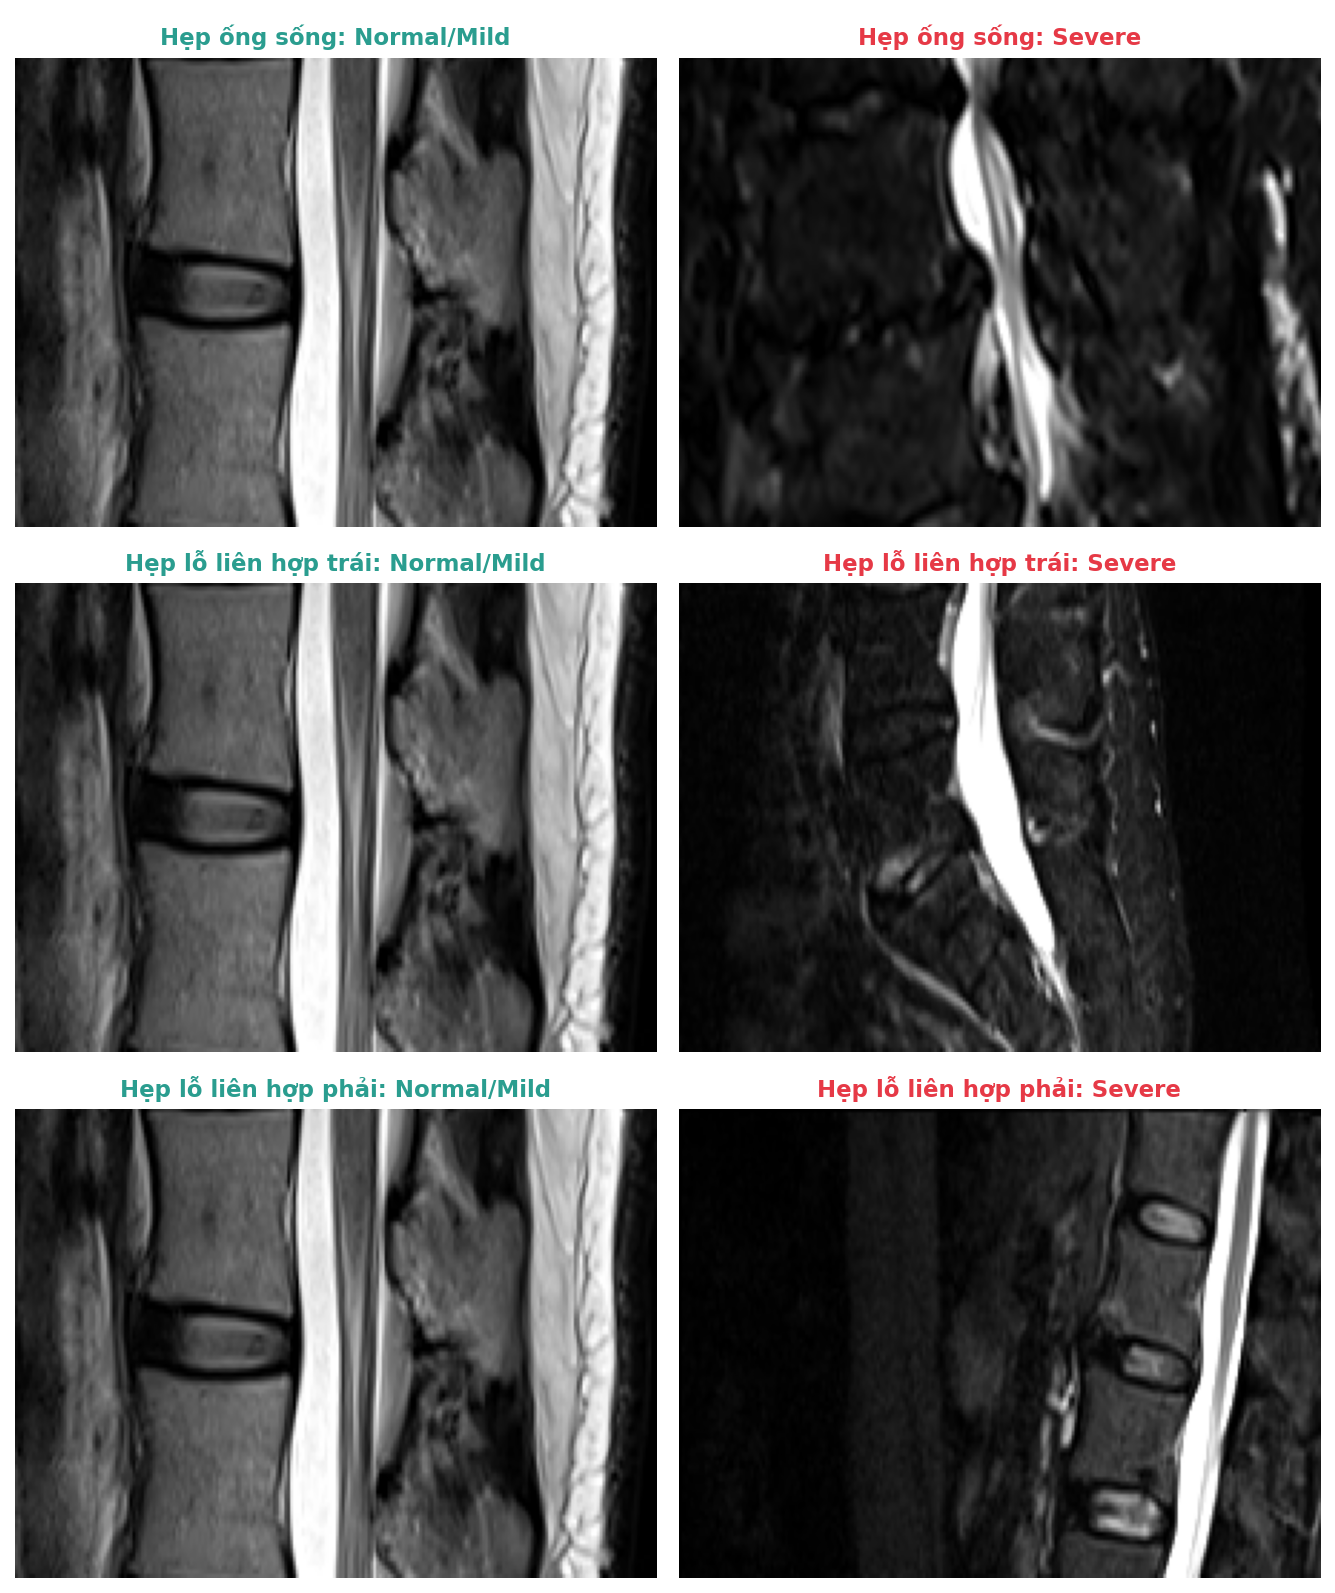
\includegraphics[height=0.62\textheight]{image/abnormality_examples.png}\\[2pt]
{\scriptsize Ví dụ Normal/Mild so với Severe cho 3 nhóm bệnh lý (RSNA 2024).}
\end{columns}
\end{frame}

\subsection{Mục tiêu và phạm vi}
\begin{frame}
\frametitle{Mục tiêu đề tài}
\begin{itemize}
    \item[\textbf{1.}] Đề xuất một pipeline giải pháp chẩn đoán đau thắt lưng; khảo sát và chọn mô hình nền cho từng mô-đun.
    \item[\textbf{2.}] Cải thiện phát hiện lớp bệnh nặng (Severe) trong bài toán mất cân bằng.
    \item[\textbf{3.}] Mở rộng nhãn bệnh mới theo hướng zero-shot, không huấn luyện lại.
    \item[\textbf{4.}] Đảm bảo tính tổng quát hóa khi chuyển sang bộ dữ liệu khác.
\end{itemize}
\end{frame}

\begin{frame}
\frametitle{Phạm vi đề tài}
\begin{itemize}
    \item[--] \textbf{Dữ liệu:} chỉ ảnh MRI cột sống thắt lưng (không xử lý X-quang/CT), chủ yếu mặt cắt Sagittal T2/STIR; chưa khai thác mặt cắt Axial.
    \item[--] \textbf{Cấu trúc giải phẫu:} đốt sống, đĩa đệm, ống sống và tủy sống.
    \item[--] \textbf{Bệnh lý đánh giá:} hẹp ống sống, hẹp lỗ liên hợp trái/phải (RSNA); mở rộng sang Pfirrmann, Modic, thoát vị, phồng đĩa đệm, trượt đốt sống (SPIDER).
\end{itemize}
\pause
\textbf{Phân chia theo giai đoạn:}
\begin{itemize}
    \item[--] \textbf{Thực tập tốt nghiệp:} khảo sát, chọn mô hình nền và tinh chỉnh mô-đun đánh giá theo hình ảnh học (radiological grading).
    \item[--] \textbf{Đồ án tốt nghiệp:} tích hợp pipeline hoàn chỉnh end-to-end và xây dựng phần mềm giao diện cho bác sĩ.
\end{itemize}
\end{frame}

%----------------------------------------------------------------------------------------
%	2. CƠ SỞ LÝ THUYẾT VÀ CÔNG TRÌNH LIÊN QUAN
%----------------------------------------------------------------------------------------
\section{Cơ sở lý thuyết và công trình liên quan}
{
    \begin{frame}[shrink]
        \frametitle{Mục lục}
        \tableofcontents[currentsection, hideothersubsections]
    \end{frame}
}

\subsection{Cơ sở lý thuyết}
\begin{frame}
\frametitle{Cơ sở lý thuyết}
\begin{itemize}\small
    \item[--] \textbf{Mất cân bằng lớp:} lớp bệnh nặng rất hiếm khiến mô hình thiên về lớp đa số $\Rightarrow$ cần augmentation, oversampling và hàm mất mát nhạy lớp hiếm (Focal Loss~\cite{lin2017focal}).
    \item[--] \textbf{Cơ chế chú ý (attention):} tự động tăng trọng số cho kênh và vùng không gian quan trọng; CBAM~\cite{woo2018cbam} kết hợp chú ý theo kênh và không gian.
    \item[--] \textbf{Mô hình thị giác--ngôn ngữ:} CLIP~\cite{radford2021clip} và BiomedCLIP~\cite{zhang2024biomedclip} học chung không gian ảnh--văn bản $\Rightarrow$ cho phép dự đoán nhãn mới bằng prompt (zero-shot).
\end{itemize}
\end{frame}

\begin{frame}
\frametitle{Attention branch (CBAM)}
\begin{figure}
\centering
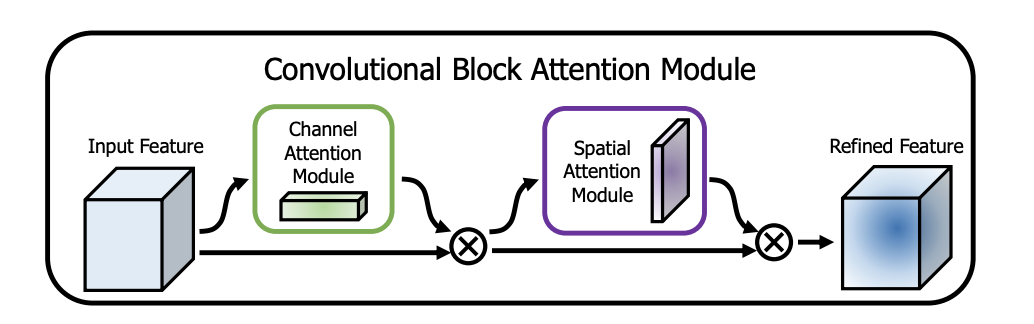
\includegraphics[width=0.84\textwidth]{image/CBAM_overview_paper.png}
\end{figure}
\begin{itemize}\small
\item[--] \textbf{Ý tưởng:} cơ chế chú ý dồn trọng số vào đúng kênh đặc trưng và vùng không gian quan trọng, thay vì xử lý đều toàn ảnh.
\item[--] \textbf{CBAM-3D:} chú ý theo \textbf{kênh} rồi \textbf{không gian}, mở rộng cho khối ảnh 3D $\Rightarrow$ hữu ích để tập trung vào vùng tổn thương nhỏ.
\end{itemize}
{\scriptsize Nguồn hình: Woo và cộng sự (2018)~\cite{woo2018cbam}.}
\end{frame}

% Slide ẩn (không trình chiếu) — chi tiết Channel & Spatial Attention; chỉ dùng để trả lời nếu hội đồng hỏi.
\iffalse
\begin{frame}
\frametitle{Chi tiết khối Channel \& Spatial Attention}
\begin{figure}
\centering
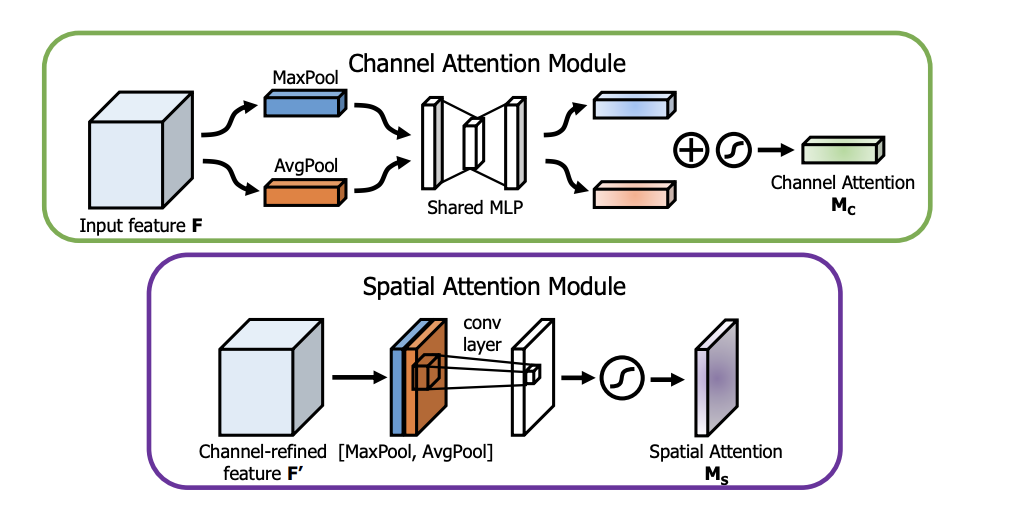
\includegraphics[width=0.86\textwidth]{image/attention_detail_cbam_paper.png}
\end{figure}
\vspace{0.3em}
\begin{itemize}\small
\item[--] \textbf{Channel attention $M_c$:} gộp avg + max pool $\to$ MLP chia sẻ $\to$ sigmoid.
\item[--] \textbf{Spatial attention $M_s$:} pool theo kênh $\to$ conv $\to$ sigmoid.
\end{itemize}
\vspace{0.2em}
{\scriptsize Nguồn hình: Woo và cộng sự (2018)~\cite{woo2018cbam}.}
\end{frame}
\fi

\begin{frame}
\frametitle{Multimodal branch (BiomedCLIP)}
\begin{figure}
\centering
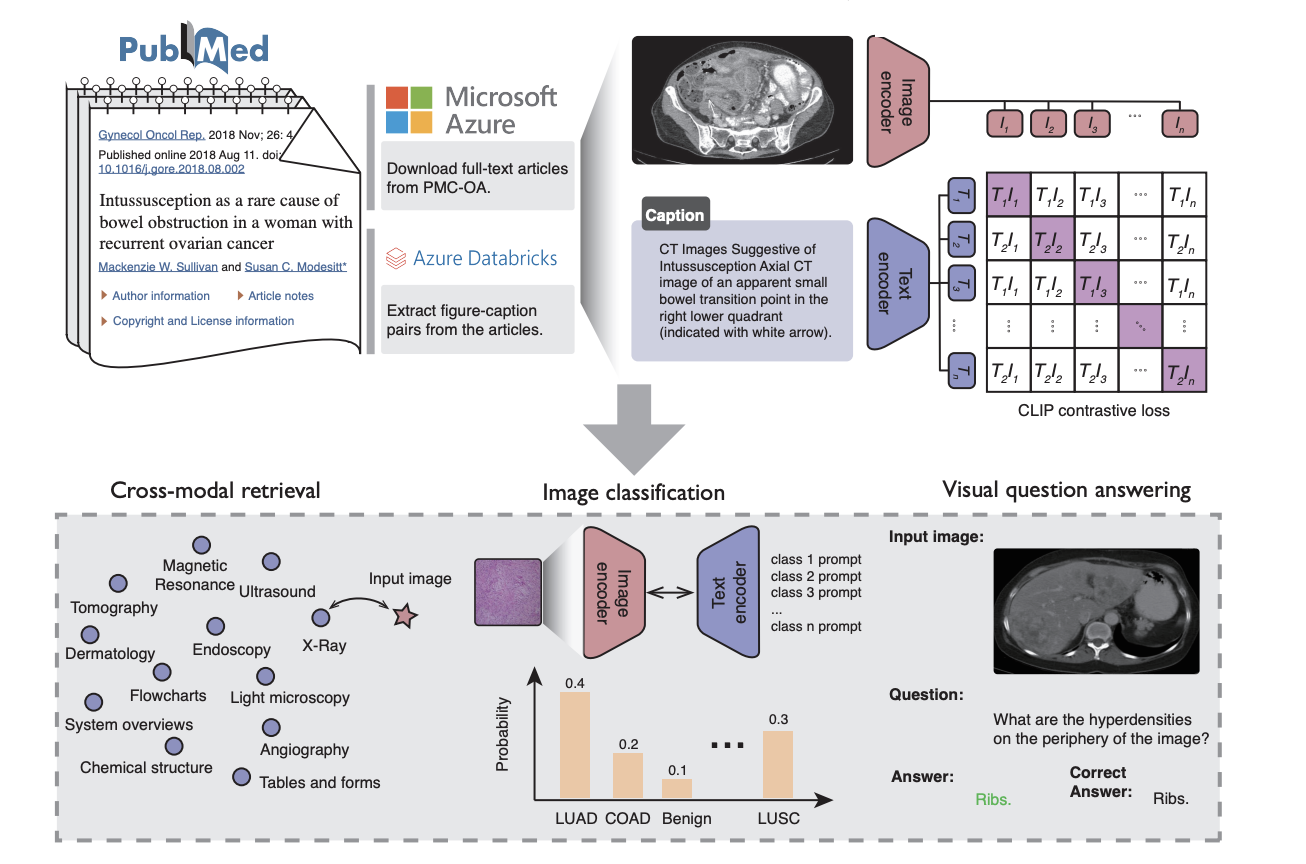
\includegraphics[width=0.74\textwidth]{image/bmc_paper.png}
\end{figure}
\vspace{-0.2em}
\begin{itemize}\scriptsize
\item[--] \textbf{Ý tưởng:} mô hình thị giác--ngôn ngữ học sẵn trên dữ liệu y khoa lớn, đặt ảnh và văn bản vào \textbf{chung không gian embedding}.
\item[--] \textbf{BiomedCLIP}~\cite{zhang2024biomedclip} (\textit{contrastive}, 15M cặp): dự đoán bằng \textbf{cosine} ảnh--prompt $\Rightarrow$ cung cấp đặc trưng y khoa tổng quát và cho phép thêm nhãn mới bằng văn bản (zero-shot).
\end{itemize}
\end{frame}

\subsection{Công trình liên quan}
\begin{frame}
\frametitle{Công trình liên quan}
\begin{table}
\centering
\footnotesize
\renewcommand{\arraystretch}{1.25}
\begin{tabular}{@{}p{3.0cm}p{3.2cm}p{3.7cm}@{}}
\toprule
\textbf{Hướng tiếp cận} & \textbf{Phương pháp} & \textbf{Mục đích / hạn chế} \\
\midrule
CNN chuyên biệt cột sống (SpineNetV2~\cite{windsor2022spinenetv2}) & ResNet-34 3D + head softmax & Chuẩn cho cột sống nhưng nhãn cố định, yếu ở lớp hiếm \\
Học giám sát đa nhãn (Ning Shen~\cite{nshen7_rsna2024}) & Ensemble CNN trên RSNA & Chính xác cao nhưng chỉ 5 nhãn, chưa được kiểm duyệt công khai \\
VLM zero-shot (MedGemma~\cite{google2025medgemma}) & Prompt ảnh--văn bản & Linh hoạt nhãn nhưng độ chính xác còn thấp \\
Cơ chế chú ý (CBAM~\cite{woo2018cbam}) & Chú ý kênh + không gian & Tập trung vào vùng tổn thương nhỏ \\
\bottomrule
\end{tabular}
\end{table}
\end{frame}

%----------------------------------------------------------------------------------------
%	3. DỮ LIỆU VÀ LỰA CHỌN MÔ HÌNH
%----------------------------------------------------------------------------------------
\section{Dữ liệu và lựa chọn mô hình}
{
    \begin{frame}[shrink]
        \frametitle{Mục lục}
        \tableofcontents[currentsection, hideothersubsections]
    \end{frame}
}

\subsection{Bộ dữ liệu}
\begin{frame}
\frametitle{Các bộ dữ liệu sử dụng}
\textbf{Đánh giá bất thường}
\begin{itemize}\small
    \item[--] \textbf{RSNA 2024}~\cite{rsna2024dataset}: MRI cột sống thắt lưng, phân mức Normal/Mild/Moderate/Severe cho hẹp ống sống và hẹp lỗ liên hợp trái/phải. Tập chính để huấn luyện và đánh giá.
    \item[--] \textbf{SPIDER}~\cite{vansluijs2022spider}: 8 nhãn bệnh (Pfirrmann, thoát vị, phồng đĩa đệm, trượt đốt sống, Modic\ldots). Dùng kiểm chứng tổng quát hóa sang dữ liệu khác.
\end{itemize}
\vspace{0.3em}
\textbf{Phân vùng cấu trúc}
\begin{itemize}\small
    \item[--] \textbf{Lumbar Spine Segmentation}~\cite{chu2015dataset}: gồm các ca chụp MRI T2 (vùng T11 đến L5), mặt nạ vùng cột sống; làm tập kiểm thử độc lập cho mô hình phân vùng.
\end{itemize}
\end{frame}

\subsection{Lựa chọn mô hình tham khảo}
\begin{frame}
\frametitle{Lựa chọn mô hình phân vùng}
\begin{table}
\centering
\small
\begin{tabular}{lcccc}
\toprule
\textbf{Tiêu chí} & \textbf{TotalSpineSeg} & \textbf{SPINEPS} & \textbf{MedCLIP-SAMv2} & \textbf{SpineNetV2} \\
\midrule
Dice Score & \textbf{70.81\%} & 58.68\% & 40.55\% & 67.82\% \\
Precision  & \textbf{97.87\%} & 52.17\% & 29.16\% & 51.76\% \\
Recall     & 56.49\% & 68.34\% & \textbf{91.98\%} & 91.79\% \\
ASSD       & \textbf{6.85 mm} & 7.48 mm & 19.50 mm & 8.04 mm \\
\bottomrule
\end{tabular}
\caption{So sánh phân vùng: TotalSpineSeg~\cite{warszawer2025totalspineseg}, SPINEPS~\cite{moller2024spineps}, MedCLIP-SAMv2~\cite{koleilat2025medclipsamv2}, SpineNetV2~\cite{windsor2022spinenetv2}.}
\end{table}
\begin{itemize}
    \item[$\rightarrow$] Chọn TotalSpineSeg: Precision 97.87\% và ASSD thấp nhất, định vị thân đốt sống chính xác để trích xuất khối liên đốt sống (IVV) chứa đĩa đệm cho grading.
\end{itemize}
\end{frame}

\begin{frame}
\frametitle{Minh hoạ output phân vùng (TotalSpineSeg)}
\begin{columns}[c]
\column{.46\textwidth}
\centering
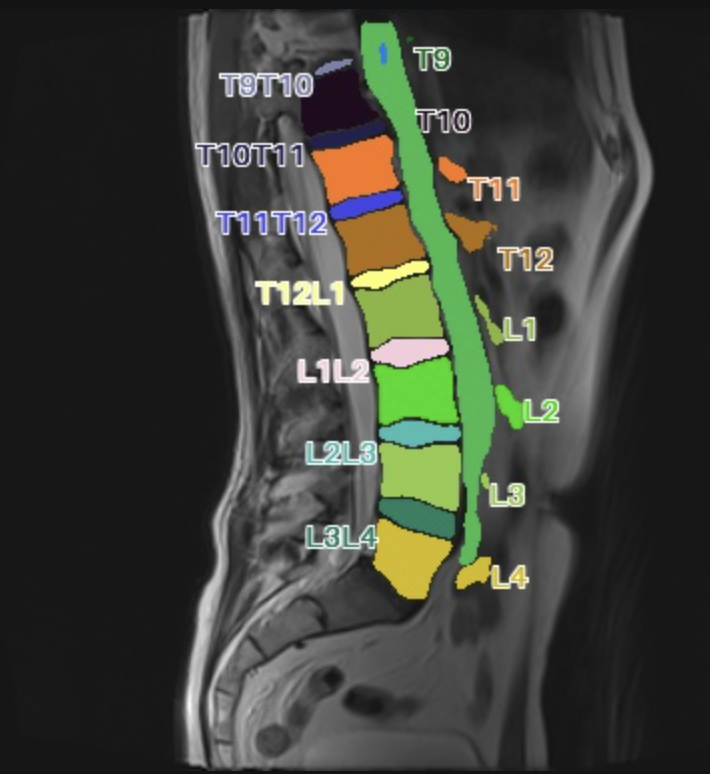
\includegraphics[height=0.62\textheight]{image/totalspineseg_output.png}
\column{.54\textwidth}
\begin{itemize}\small
    \item[--] TotalSpineSeg phân vùng và gán nhãn từng đốt sống, đĩa đệm trên mặt cắt Sagittal.
    \item[--] Mặt nạ này dùng để định vị khối liên đốt sống (IVV) chứa đĩa đệm cho mô-đun đánh giá ở giai đoạn sau.
\end{itemize}
\end{columns}
\end{frame}

\begin{frame}
\frametitle{Lựa chọn mô-đun đánh giá bất thường}
\begin{table}
\centering
\small
\renewcommand{\arraystretch}{1.2}
\begin{tabular}{lcccc}
\toprule
\textbf{Mô hình} & \textbf{Accuracy} & \textbf{Precision} & \textbf{Recall} & \textbf{F1} \\
\midrule
Ning Shen~\cite{nshen7_rsna2024}   & \textbf{80.8\%} & \textbf{77.7\%} & \textbf{84.2\%} & \textbf{80.7\%} \\
SpineNetV2~\cite{windsor2022spinenetv2}  & 76.5\% & 74.9\% & 80.4\% & 77.5\% \\
MedGemma~\cite{google2025medgemma}    & 38.7\% & 50.1\% & 11.8\% & 18.6\% \\
\bottomrule
\end{tabular}
\caption{So sánh phát hiện bất thường (trung bình 3 nhóm bệnh).}
\end{table}
\begin{itemize}
    \item[$\rightarrow$] Chọn \textbf{SpineNetV2} làm backbone: chuyên biệt cột sống, nhiều nhãn, mã nguồn mở. Ning Shen mạnh hơn nhưng chỉ 5 nhãn và chưa được kiểm duyệt công khai; MedGemma Recall quá thấp ($\sim$12\%).
\end{itemize}
\end{frame}

\begin{frame}
\frametitle{Các thách thức chính}
\begin{columns}[c]
\column{.54\textwidth}
\begin{itemize}\small
    \item[\textbf{1.}] \textbf{Mất cân bằng lớp:} lớp Severe quá hiếm ($\sim$4\%) $\Rightarrow$ Recall lớp Severe rất thấp, dễ bỏ sót ca nặng.
    \item[\textbf{2.}] \textbf{Mở rộng nhãn (zero-shot):} thêm nhãn bệnh mới mà không huấn luyện lại; head phân loại cố định không làm được.
    \item[\textbf{3.}] \textbf{Tổng quát hóa:} mô hình phải giữ được hiệu năng khi chuyển sang bộ dữ liệu khác.
\end{itemize}
\column{.46\textwidth}
\centering
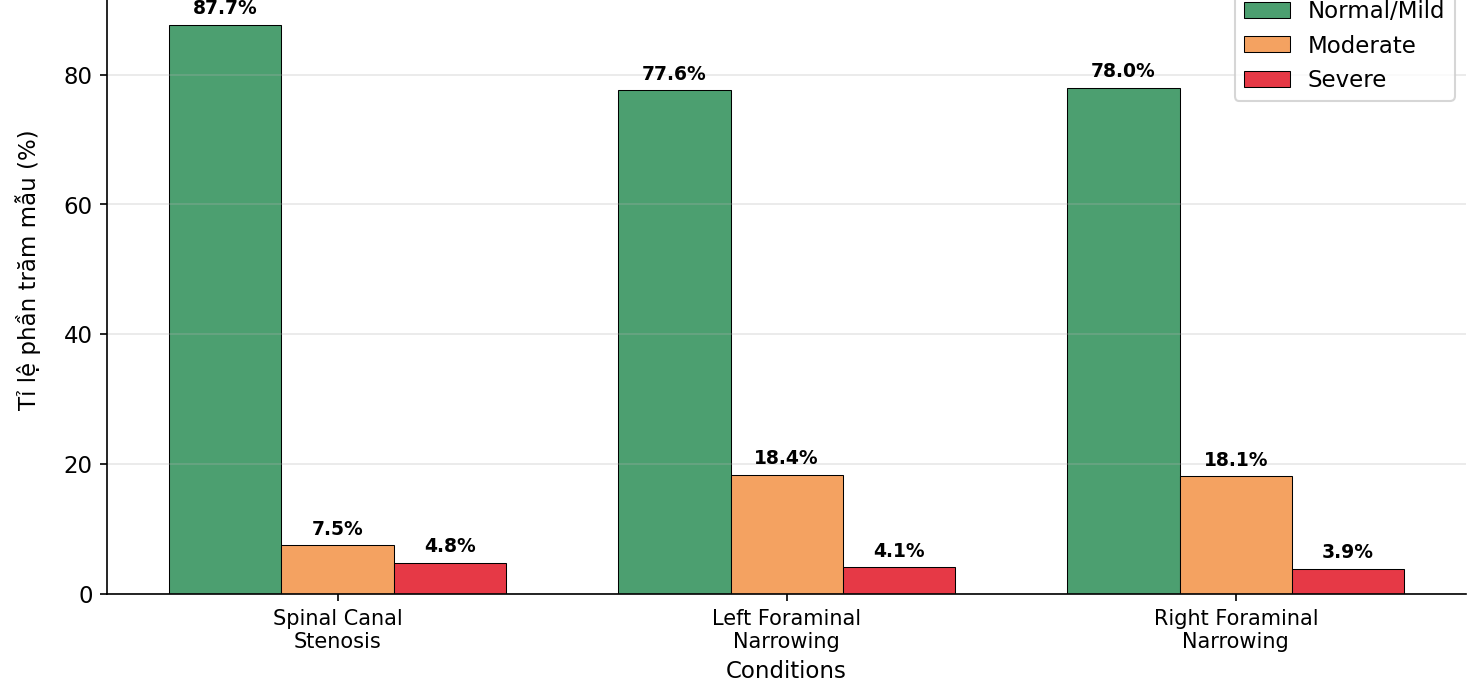
\includegraphics[width=\linewidth]{image/rsna_class_distribution_nobanner.png}\\[2pt]
{\scriptsize Phân bố lớp RSNA 2024 (minh họa thách thức 1).}
\end{columns}
\end{frame}

%----------------------------------------------------------------------------------------
%	4. MÔ HÌNH ĐỀ XUẤT
%----------------------------------------------------------------------------------------
\section{Mô hình đề xuất}
{
    \begin{frame}[shrink]
        \frametitle{Mục lục}
        \tableofcontents[currentsection, hideothersubsections]
    \end{frame}
}

\subsection{Kiến trúc tổng thể}
\begin{frame}
\frametitle{Pipeline giải pháp chẩn đoán đau thắt lưng}
\textbf{Đề xuất} một pipeline hai mô-đun nối tiếp cho chẩn đoán đau thắt lưng:
\begin{figure}
\centering
\resizebox{\textwidth}{!}{%
\begin{tikzpicture}[
    box/.style={rectangle, draw=blue!70, fill=blue!8, rounded corners, minimum width=1.9cm, minimum height=0.95cm, align=center, font=\footnotesize, thick},
    dataout/.style={rectangle, draw=green!50!black, fill=green!12, rounded corners, minimum width=1.9cm, minimum height=0.95cm, align=center, font=\footnotesize, thick},
    plan/.style={rectangle, draw=gray, dashed, fill=gray!8, rounded corners, minimum width=2.0cm, minimum height=0.95cm, align=center, font=\footnotesize, thick},
    a/.style={->, thick, blue!70!black},
    pa/.style={->, thick, gray, dashed}
]
    \node[box] (in)   at (0,0)    {Ảnh MRI};
    \node[box] (seg)  at (2.6,0)  {Phân vùng\\\scriptsize TotalSpineSeg};
    \node[dataout] (mask) at (5.2,0)  {Mặt nạ};
    \node[box] (gr)   at (7.8,0)  {Đánh giá\\\scriptsize Hybrid grading};
    \node[dataout] (lb)   at (10.4,0) {Nhãn bệnh lý};
    \node[plan](sw)   at (13.0,0) {Phần mềm\\\scriptsize giao diện};
    \draw[a] (in) -- (seg);
    \draw[a] (seg) -- (mask);
    \draw[pa] (mask) -- node[above,font=\scriptsize,text=gray]{IVV} (gr);
    \draw[a] (gr) -- (lb);
    \draw[pa] (lb) -- (sw);
    \draw[a] (in) to[bend right=30] (gr);
\end{tikzpicture}}
\caption{Pipeline đề xuất. \textcolor{blue!70!black}{Nét liền} = đã làm ở giai đoạn thực tập; \textcolor{gray}{nét đứt xám} = chưa làm (kế hoạch Đồ án tốt nghiệp).}
\end{figure}
\begin{itemize}
    \item[--] Luồng mục tiêu: MRI $\rightarrow$ phân vùng $\rightarrow$ mặt nạ định vị khối liên đốt sống (IVV) $\rightarrow$ đánh giá $\rightarrow$ phần mềm.
    \item[--] Hiện trạng thực tập: hai mô-đun chạy độc lập, grading nhận ảnh MRI trực tiếp (nét liền cong).
\end{itemize}
\end{frame}

\subsection{Kiến trúc Hybrid hai nhánh}
\begin{frame}
\frametitle{Kiến trúc Hybrid hai nhánh (đề xuất)}
\begin{figure}
    \centering
    
\includegraphics[width=\textwidth]{image/hybrid_arch_generic.pdf}
\end{figure}
\vspace{0.4em}
\begin{itemize}\footnotesize
    \item[--] Ghép \textbf{hai nhánh bổ trợ}: chú ý cục bộ 3D (Attention) + prior y khoa tổng quát (Multimodal).
    \item[--] \textbf{Fusion head} hợp nhất hai đặc trưng, rồi \textbf{đầu cosine} đối sánh với prompt văn bản.
    \item[--] Nhờ đầu cosine--prompt: hỗ trợ cả nhãn đã học lẫn \textbf{thêm nhãn mới zero-shot}.
\end{itemize}
\end{frame}

\subsection{Huấn luyện và suy diễn}
\begin{frame}
\frametitle{Giai đoạn huấn luyện và suy diễn}
\begin{columns}[T]
\column{.5\textwidth}
\centering{\small\textbf{Huấn luyện}}\\[3pt]
\resizebox{0.94\linewidth}{!}{%
\begin{tikzpicture}[font=\sffamily\scriptsize,>={Stealth[round]},
  io/.style={rectangle,rounded corners=2pt,draw=black!55,fill=black!7,align=center,inner sep=3pt},
  tr/.style={rectangle,rounded corners=2pt,draw=blue!60!black,fill=blue!16,align=center,inner sep=3pt},
  fz/.style={rectangle,rounded corners=2pt,draw=black!45,fill=black!12,align=center,inner sep=3pt},
  loss/.style={rectangle,rounded corners=2pt,draw=red!55!black,fill=red!12,align=center,inner sep=3pt},
  ar/.style={->,thick,black!70}]
\node[io](v){Khối ảnh MRI};
\node[io,below=4mm of v](aug){Augmentation};
\node[fz,below=9mm of aug,xshift=-15mm](b1){CBAM-3D\\ResNet-34};
\node[fz,below=9mm of aug,xshift=15mm](b2){BiomedCLIP\\ViT-B/16};
\node[tr,below=22mm of aug](cat){Concat 1024 $\to$ Fusion MLP};
\node[tr,below=4mm of cat](head){Cosine head};
\node[loss,below=4mm of head](loss){Loss: Focal + Uncertainty};
\draw[ar](v)--(aug);
\draw[ar](aug)--(b1);\draw[ar](aug)--(b2);
\draw[ar](b1)--(cat);\draw[ar](b2)--(cat);
\draw[ar](cat)--(head);\draw[ar](head)--(loss);
\draw[->,thick,red!55!black,dashed] (loss.east) to[out=0,in=0,looseness=1.8] node[pos=0.5,right=2pt,font=\tiny,text=red!55!black]{backprop} (cat.east);
\end{tikzpicture}}
\column{.5\textwidth}
\centering{\small\textbf{Suy diễn}}\\[3pt]
\resizebox{0.94\linewidth}{!}{%
\begin{tikzpicture}[font=\sffamily\scriptsize,>={Stealth[round]},
  io/.style={rectangle,rounded corners=2pt,draw=black!55,fill=black!7,align=center,inner sep=3pt},
  tr/.style={rectangle,rounded corners=2pt,draw=blue!60!black,fill=blue!16,align=center,inner sep=3pt},
  fz/.style={rectangle,rounded corners=2pt,draw=black!45,fill=black!12,align=center,inner sep=3pt},
  obox/.style={rectangle,rounded corners=2pt,draw=green!50!black,fill=green!14,align=center,inner sep=3pt},
  ar/.style={->,thick,black!70}]
\node[io](v){Khối ảnh MRI};
\node[tr,below=9mm of v,xshift=-15mm](b1){CBAM-3D\\ResNet-34};
\node[fz,below=9mm of v,xshift=15mm](b2){BiomedCLIP\\ViT-B/16};
\node[tr,below=22mm of v](cat){Concat 1024 $\to$ Fusion MLP};
\node[tr,below=4mm of cat](head){Classification heads};
\node[obox,below=4mm of head](o){Output: xác suất + nhãn};
\draw[ar](v)--(b1);\draw[ar](v)--(b2);
\draw[ar](b1)--(cat);\draw[ar](b2)--(cat);
\draw[ar](cat)--(head);\draw[ar](head)--(o);
\end{tikzpicture}}
\end{columns}
\vspace{0.3em}
{\footnotesize Huấn luyện: dùng augmentation + Focal loss để xử lý mất cân bằng, rồi lan truyền ngược. Suy diễn: chỉ forward pass, xuất xác suất và nhãn dự đoán.}
\end{frame}

%----------------------------------------------------------------------------------------
%	5. KẾT QUẢ THỰC NGHIỆM
%----------------------------------------------------------------------------------------
\section{Kết quả thực nghiệm}
{
    \begin{frame}[shrink]
        \frametitle{Mục lục}
        \tableofcontents[currentsection, hideothersubsections]
    \end{frame}
}

\subsection{Thiết lập thực nghiệm}
\begin{frame}
\frametitle{Thiết lập thực nghiệm}
{\footnotesize \textbf{Hai nhóm thực nghiệm:} (1) lựa chọn mô hình nền (mục trước); (2) xác thực đóng góp grading (mục này).}
\begin{table}
\centering
\renewcommand{\arraystretch}{1.3}
\small
\begin{tabular}{@{}l p{8.1cm}@{}}
\toprule
\textbf{Hạng mục} & \textbf{Cấu hình} \\
\midrule
RSNA 2024~\cite{rsna2024dataset} & $\sim$1\,800 BN train / $\sim$225 BN val; Sagittal T2/STIR; 3 nhóm bệnh \\
SPIDER~\cite{vansluijs2022spider} & 8 nhãn; transfer learning (kiểm chứng tổng quát hóa) \\
Ablation & SpineNetV2 / CBAM / BMC-only / Hybrid \\
Phần cứng & NVIDIA RTX 4090 (24GB), Vast.ai \\
Framework & PyTorch 2.0, Python 3.10 \\
Tối ưu & AdamW, batch 32; Focal + Uncertainty + oversampling \\
Đánh giá & macro R/P/F1/AUC/AUPRC + lớp Severe \\
\bottomrule
\end{tabular}
\end{table}
\end{frame}

\subsection{Kết quả tinh chỉnh trên RSNA}
\begin{frame}
\frametitle{Kết quả tổng hợp trên RSNA 2024}
\begin{table}
\centering
\small
\begin{tabular}{lcccc}
\toprule
\textbf{Chỉ số} & \textbf{SpineNetV2} & \textbf{CBAM} & \textbf{BMC-only} & \textbf{Hybrid (ours)} \\
\midrule
Mean Accuracy   & \textbf{0.814} & 0.690 & 0.692 & 0.721 \\
Mean F1 (macro) & 0.420 & 0.502 & 0.464 & \textbf{0.528} \\
Mean AUC        & 0.826 & 0.822 & 0.812 & \textbf{0.837} \\
Mean AUPRC      & 0.523 & 0.519 & 0.482 & \textbf{0.526} \\
\midrule
\multicolumn{5}{l}{\textit{Lớp Severe (lớp focus lâm sàng)}} \\
Severe Recall   & 0.115 & 0.370 & 0.245 & \textbf{0.464} \\
Severe F1       & 0.149 & 0.304 & 0.229 & \textbf{0.343} \\
Severe AUC      & 0.860 & 0.886 & 0.874 & \textbf{0.896} \\
Severe AUPRC    & 0.276 & 0.319 & 0.218 & \textbf{0.321} \\
\bottomrule
\end{tabular}
\caption{Kết quả trung bình và lớp Severe của 4 cấu hình trên RSNA 2024.}
\end{table}
\begin{itemize}
    \item[$\rightarrow$] SpineNetV2 cao nhất ở Accuracy (do thiên về lớp đa số); Hybrid đánh đổi $\sim$9\% Accuracy để dẫn đầu F1/AUC/AUPRC và đặc biệt là lớp Severe (xem chi tiết bên dưới).
\end{itemize}
\end{frame}

\begin{frame}
\frametitle{Kết quả chi tiết theo lớp trên RSNA 2024}
\begin{table}
\centering
\scriptsize
\setlength{\tabcolsep}{4pt}
\renewcommand{\arraystretch}{1.05}
\begin{tabular}{llccccc}
\toprule
\textbf{Lớp} & \textbf{Cấu hình} & R & P & F1 & AUC & AUPRC \\
\midrule
\multirow{4}{*}{Normal/Mild}
 & SpineNetV2 & \textbf{0.963} & 0.840 & \textbf{0.897} & 0.829 & 0.948 \\
 & CBAM       & 0.693 & \textbf{0.949} & 0.791 & 0.848 & 0.949 \\
 & BMC-only   & 0.709 & 0.934 & 0.801 & 0.828 & 0.950 \\
 & Hybrid     & 0.746 & 0.937 & 0.825 & \textbf{0.861} & \textbf{0.957} \\
\midrule
\multirow{4}{*}{Moderate}
 & SpineNetV2 & 0.173 & \textbf{0.424} & 0.240 & \textbf{0.790} & \textbf{0.345} \\
 & CBAM       & \textbf{0.652} & 0.310 & 0.411 & 0.732 & 0.288 \\
 & BMC-only   & 0.563 & 0.280 & 0.360 & 0.733 & 0.278 \\
 & Hybrid     & 0.564 & 0.341 & \textbf{0.415} & 0.753 & 0.300 \\
\midrule
\multirow{4}{*}{\textbf{Severe}}
 & SpineNetV2 & 0.115 & 0.212 & 0.149 & 0.860 & 0.276 \\
 & CBAM       & 0.370 & 0.272 & 0.304 & 0.886 & 0.319 \\
 & BMC-only   & 0.245 & 0.211 & 0.229 & 0.874 & 0.218 \\
 & Hybrid     & \textbf{0.464} & \textbf{0.273} & \textbf{0.343} & \textbf{0.896} & \textbf{0.321} \\
\bottomrule
\end{tabular}
\caption{Chi tiết per-class trên RSNA 2024 (Hybrid: cấu hình đề xuất / ours).}
\end{table}
\begin{itemize}
    \item[$\rightarrow$] Lớp Severe: Hybrid thắng cả 5 chỉ số, Severe Recall 11.5\% $\to$ 46.4\% (gấp $\sim$4 lần).
\end{itemize}
\end{frame}

\subsection{Khả năng diễn giải}
\begin{frame}
\frametitle{Trực quan hóa vùng chú ý (Grad-CAM)}
\begin{figure}
\centering
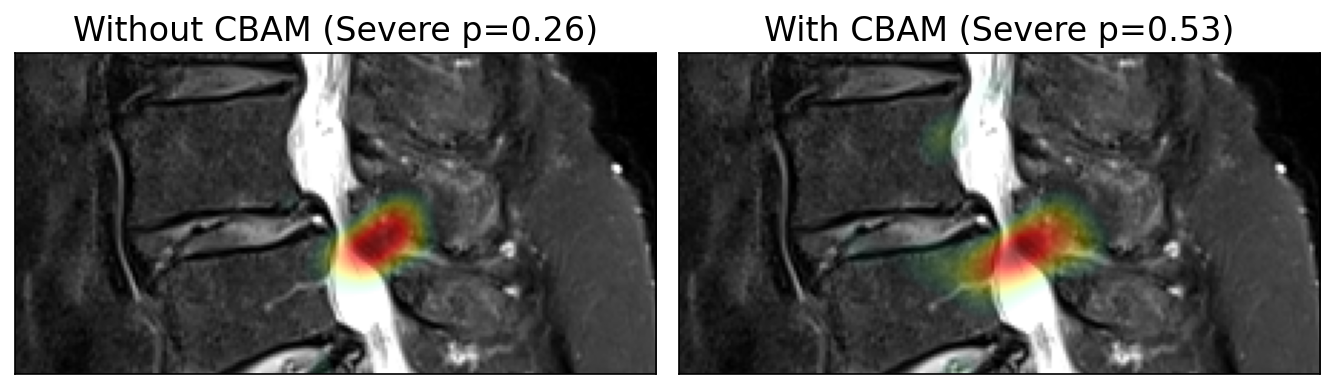
\includegraphics[width=0.78\textwidth]{image/grad_cam_nocbam_vs_cbam.png}
\caption{Grad-CAM ca Severe hẹp ống sống (L4-L5): không CBAM so với có CBAM.}
\end{figure}
\begin{itemize}\footnotesize
    \item[$\rightarrow$] Không CBAM: chú ý dàn trải, xác suất Severe thấp (p=0.26). Có CBAM: tập trung đúng vùng đĩa--ống sống, p=0.53.
\end{itemize}
\end{frame}

\subsection{Mở rộng nhãn zero-shot}
\begin{frame}
\frametitle{Mở rộng nhãn zero-shot trên SPIDER}
\begin{columns}[t]
\column{.5\textwidth}
\small
Cho phép thêm nhãn bệnh mới chỉ bằng cách đổi prompt văn bản (zero-shot), không cần huấn luyện lại trên SPIDER.
\begin{itemize}\small
    \item[$\rightarrow$] Baseline/CBAM không làm được vì head phân loại cố định 3 lớp.
\end{itemize}
\column{.5\textwidth}
\begin{table}
\centering
\footnotesize
\begin{tabular}{lcc}
\toprule
\textbf{Nhãn SPIDER} & \textbf{F1} & \textbf{AUC} \\
\midrule
Disc bulging        & \textbf{0.613} & 0.829 \\
Disc herniation     & 0.563 & 0.772 \\
Disc narrowing      & 0.586 & 0.834 \\
\midrule
Lower endplate      & 0.468 & 0.738 \\
Upper endplate      & 0.467 & 0.740 \\
Pfirrmann (5 lớp)   & 0.155 & 0.687 \\
Modic (4 lớp)       & 0.018 & 0.454 \\
Spondylolisthesis   & 0.028 & 0.807 \\
\midrule
\textbf{Trung bình (8)} & \textbf{0.362} & \textbf{0.733} \\
\bottomrule
\end{tabular}
\end{table}
\end{columns}
\end{frame}

\subsection{Tổng quát hóa trên SPIDER}
\begin{frame}
\frametitle{Kết quả tổng hợp trên SPIDER}
\begin{table}
\centering
\small
\begin{tabular}{lcccc}
\toprule
\textbf{Chỉ số} & \textbf{SpineNetV2} & \textbf{CBAM} & \textbf{BMC-only} & \textbf{Hybrid (ours)} \\
\midrule
Mean Accuracy (\%) & \textbf{80.23} & 79.27 & 76.12 & 78.30 \\
Mean F1 (macro)    & 0.646 & 0.619 & 0.613 & \textbf{0.653} \\
Mean AUC           & 0.842 & 0.824 & 0.808 & \textbf{0.846} \\
Mean AUPRC         & \textbf{0.633} & 0.580 & 0.544 & 0.611 \\
\bottomrule
\end{tabular}
\caption{Kết quả trung bình 4 cấu hình trên SPIDER (có tinh chỉnh).}
\end{table}
\begin{itemize}
    \item[$\rightarrow$] Có tinh chỉnh, kết quả cao hơn hẳn zero-shot (Mean F1 0.653 so với 0.362).
\end{itemize}
\end{frame}

\begin{frame}
\frametitle{Kết quả chi tiết trên SPIDER}
\begin{table}
\centering
\scriptsize
\setlength{\tabcolsep}{3.5pt}
\resizebox{\textwidth}{!}{%
\begin{tabular}{lccccccccccc}
\toprule
& \multicolumn{5}{c}{\textbf{SpineNetV2}} & & \multicolumn{5}{c}{\textbf{Hybrid (ours)}} \\
\cmidrule(lr){2-6}\cmidrule(lr){8-12}
\textbf{Nhóm bệnh} & R & P & F1 & AUC & AUPRC & & R & P & F1 & AUC & AUPRC \\
\midrule
Modic             & 0.374 & \textbf{0.383} & 0.376 & 0.731 & \textbf{0.545} & & \textbf{0.382} & 0.377 & \textbf{0.379} & \textbf{0.827} & 0.500 \\
Disc narrowing    & 0.820 & \textbf{0.828} & 0.823 & \textbf{0.927} & 0.882 & & \textbf{0.836} & 0.827 & \textbf{0.831} & 0.916 & \textbf{0.884} \\
Spondylolisthesis & 0.597 & \textbf{0.793} & \textbf{0.632} & \textbf{0.826} & \textbf{0.325} & & \textbf{0.633} & 0.607 & 0.613 & 0.815 & 0.302 \\
UP endplate       & 0.727 & 0.746 & 0.728 & 0.820 & \textbf{0.753} & & \textbf{0.753} & \textbf{0.748} & \textbf{0.749} & \textbf{0.828} & 0.751 \\
LOW endplate      & \textbf{0.754} & \textbf{0.764} & \textbf{0.757} & 0.823 & \textbf{0.775} & & 0.743 & 0.745 & 0.744 & \textbf{0.826} & 0.763 \\
Disc herniation   & 0.500 & 0.470 & 0.485 & 0.852 & \textbf{0.271} & & \textbf{0.636} & \textbf{0.592} & \textbf{0.601} & \textbf{0.860} & 0.248 \\
Disc bulging      & 0.778 & 0.779 & 0.777 & \textbf{0.874} & 0.840 & & \textbf{0.796} & \textbf{0.794} & \textbf{0.792} & 0.873 & \textbf{0.851} \\
\bottomrule
\end{tabular}}
\caption{Recall/Precision/F1/AUC/AUPRC theo từng nhóm bệnh trên SPIDER.}
\end{table}
\begin{itemize}
    \item[$\rightarrow$] Hybrid cải thiện Recall/F1/AUC ở phần lớn nhóm bệnh.
\end{itemize}
\end{frame}

%----------------------------------------------------------------------------------------
%	6. KẾT LUẬN
%----------------------------------------------------------------------------------------
\section{Kết luận và hướng phát triển}
{
    \begin{frame}[shrink]
        \frametitle{Mục lục}
        \tableofcontents[currentsection, hideothersubsections]
    \end{frame}
}

\begin{frame}
\frametitle{Đóng góp chính}
Bên cạnh việc khảo sát và lựa chọn mô hình nền cho cả hai mô-đun của hệ thống, đề tài có \textbf{3 đóng góp chính}:
\begin{itemize}
    \item[1.] \textbf{Đề xuất kiến trúc Hybrid hai nhánh} (Attention + Multimodal) kết hợp \textbf{kỹ thuật xử lý mất cân bằng} (augmentation, oversampling, Focal + Uncertainty loss) cho mô-đun đánh giá, nâng Recall lớp Severe từ \textbf{11.5\% lên 46.4\%} ($\sim$4 lần).
    \item[2.] \textbf{Cơ chế mở rộng nhãn theo hướng zero-shot:} bổ sung nhãn bệnh mới qua mô tả văn bản, không huấn luyện lại.
    \item[3.] \textbf{Đánh giá khả năng tổng quát hóa liên tập dữ liệu} (RSNA $\to$ SPIDER): Hybrid duy trì hiệu năng ổn định.
\end{itemize}
\end{frame}

\begin{frame}
\frametitle{Hạn chế}
\begin{itemize}
    \item[--] Hai mô-đun phân vùng và đánh giá còn chạy độc lập, chưa tích hợp thành pipeline hoàn chỉnh.
    \item[--] Mô hình mới khai thác mặt cắt Sagittal, chưa dùng mặt cắt Axial.
    \item[--] Chỉ số đo lường tuyệt đối còn thấp (ví dụ Severe F1 $\sim$0.34; vài nhãn SPIDER khó như Modic/Pfirrmann còn yếu) -- cần cải thiện thêm.
\end{itemize}
\end{frame}

\begin{frame}
\frametitle{Kế hoạch giai đoạn Đồ án tốt nghiệp}
\begin{table}
\centering
\begin{tabular}{c p{6.2cm} c}
\toprule
\textbf{GĐ} & \textbf{Nội dung} & \textbf{Thời lượng} \\
\midrule
1 & Tích hợp pipeline end-to-end (mặt nạ định vị IVV) & 3 tuần \\
2 & Xây dựng phần mềm giao diện cho bác sĩ & 3 tuần \\
3 & Bổ sung cơ chế dùng phản hồi của bác sĩ để mô hình tự cải thiện & 3 tuần \\
4 & Viết Đồ án tốt nghiệp và chuẩn bị bảo vệ & 3 tuần \\
\bottomrule
\end{tabular}
\caption{Kế hoạch thực hiện trong giai đoạn Đồ án tốt nghiệp.}
\end{table}
\end{frame}

%----------------------------------------------------------------------------------------
\section{Tài liệu tham khảo}
\begin{frame}[allowframebreaks]
\frametitle{Tài liệu tham khảo}
\printbibliography
\end{frame}

%------------------------------------------------
\begin{frame}
\huge{\centerline{Xin cảm ơn quý thầy cô đã lắng nghe!}}
\end{frame}

\appendix
\begin{frame}
\frametitle{Phụ lục: số tham số mô hình}
\begin{table}
\centering
\begin{tabular}{lcc}
\toprule
\textbf{Thành phần} & \textbf{Số tham số} & \textbf{Trạng thái} \\
\midrule
CBAM-3D ResNet-34 & 21.3M & Frozen (pretrained) \\
BiomedCLIP ViT-B/16 & 86.2M & Frozen \\
Khối hợp nhất (fusion + cosine) & $\sim$0.5M & Huấn luyện \\
\bottomrule
\end{tabular}
\caption{Phân bổ tham số trong kiến trúc Hybrid.}
\end{table}
\end{frame}

\begin{frame}
\frametitle{Phụ lục: chi phí tính toán \& hội tụ}
\begin{table}
\centering
\begin{tabular}{lcc}
\toprule
\textbf{Cấu hình} & \textbf{Thời gian train} & \textbf{Suy luận (ms/mẫu)} \\
\midrule
Baseline   & 16.4 phút & 62.0 \\
CBAM       & 56.0 phút & 62.4 \\
Hybrid (thêm trên nền CBAM) & +24.8 phút & 61.6 \\
\bottomrule
\end{tabular}
\caption{Chi phí huấn luyện và suy luận grading trên RSNA 2024 (một GPU RTX 4090).}
\end{table}
\begin{itemize}\footnotesize
    \item[--] Chọn checkpoint theo validation (early stopping), không lấy epoch cuối.
    \item[--] Hybrid là \textbf{bước 2}: nạp checkpoint CBAM (frozen) rồi chỉ huấn luyện khối hợp nhất $\Rightarrow$ 24.8 phút là chi phí \textbf{huấn luyện thêm} (chưa gồm bước 1 train CBAM).
    \item[--] Suy luận $\sim$62 ms/mẫu cho cả ba cấu hình.
\end{itemize}
\end{frame}

\begin{frame}
\frametitle{Phụ lục: vị trí CBAM trên backbone ResNet-34}
\begin{figure}
\centering
\resizebox{\textwidth}{!}{%
\begin{tikzpicture}[font=\sffamily\scriptsize,>={Stealth[round]},
  io/.style={rectangle,rounded corners=2pt,draw=black!55,fill=black!7,align=center,inner sep=3pt},
  res/.style={rectangle,rounded corners=2pt,draw=blue!60!black,fill=blue!16,align=center,inner sep=3pt,minimum height=10mm},
  cb/.style={rectangle,rounded corners=2pt,draw=orange!80!black,fill=orange!20,align=center,inner sep=3pt,minimum height=10mm},
  ar/.style={->,thick,black!70}]
\node[io](in){Khối ảnh\\$9{\times}112{\times}224$};
\node[io,right=4mm of in](stem){Conv1\\+ MaxPool};
\node[res,right=4mm of stem](l1){Layer1};
\node[cb,right=2.5mm of l1](c1){CBAM};
\node[res,right=2.5mm of c1](l2){Layer2};
\node[cb,right=2.5mm of l2](c2){CBAM};
\node[res,right=2.5mm of c2](l3){Layer3};
\node[cb,right=2.5mm of l3](c3){CBAM};
\node[res,right=2.5mm of c3](l4){Layer4};
\node[cb,right=2.5mm of l4](c4){CBAM};
\node[io,right=4mm of c4](gap){GAP\\$\to$ 512-d};
\draw[ar](in)--(stem);\draw[ar](stem)--(l1);
\draw[ar](l1)--(c1);\draw[ar](c1)--(l2);\draw[ar](l2)--(c2);\draw[ar](c2)--(l3);
\draw[ar](l3)--(c3);\draw[ar](c3)--(l4);\draw[ar](l4)--(c4);\draw[ar](c4)--(gap);
\end{tikzpicture}}
\caption{CBAM (cam) được chèn \textbf{sau mỗi stage} của backbone ResNet-34 3D (xanh) trong nhánh grading; đầu ra là vector đặc trưng 512 chiều đưa vào khối hợp nhất.}
\end{figure}
{\footnotesize Backbone giữ nguyên cấu trúc ResNet-34 của SpineNetV2~\cite{windsor2022spinenetv2}; CBAM~\cite{woo2018cbam} chỉ thêm $\sim$1\% tham số nhưng giúp khu trú vùng tổn thương.}
\end{frame}

\begin{frame}
\frametitle{Phụ lục: kiến trúc SpineNetV2 (baseline)}
\begin{figure}
\centering
\resizebox{\textwidth}{!}{%
\begin{tikzpicture}[font=\sffamily\scriptsize,>={Stealth[round]},
  io/.style={rectangle,rounded corners=2pt,draw=black!55,fill=black!7,align=center,inner sep=3pt},
  res/.style={rectangle,rounded corners=2pt,draw=blue!60!black,fill=blue!16,align=center,inner sep=3pt,minimum height=10mm},
  hd/.style={rectangle,rounded corners=2pt,draw=teal!65!black,fill=teal!14,align=center,inner sep=3pt,minimum height=10mm},
  ob/.style={rectangle,rounded corners=2pt,draw=green!50!black,fill=green!16,align=center,inner sep=3pt},
  ar/.style={->,thick,black!70}]
\node[io](in){Khối ảnh\\$9{\times}112{\times}224$};
\node[io,right=3.5mm of in](stem){Conv1\\+ MaxPool};
\node[res,right=3.5mm of stem](l1){Layer1};
\node[res,right=2.2mm of l1](l2){Layer2};
\node[res,right=2.2mm of l2](l3){Layer3};
\node[res,right=2.2mm of l3](l4){Layer4};
\node[io,right=3.5mm of l4](gap){GAP\\$\to$ 512-d};
\node[hd,right=3.5mm of gap](head){Linear head\\+ Softmax};
\node[ob,right=3.5mm of head](o){Lớp \textbf{cố định}:\\Normal/Mild,\\Moderate, Severe};
\draw[ar](in)--(stem);\draw[ar](stem)--(l1);\draw[ar](l1)--(l2);\draw[ar](l2)--(l3);
\draw[ar](l3)--(l4);\draw[ar](l4)--(gap);\draw[ar](gap)--(head);\draw[ar](head)--(o);
\node[font=\sffamily\scriptsize,text=blue!50!black,above=1mm of l2,xshift=6mm]{ResNet-34 (4 stage, không CBAM)};
\end{tikzpicture}}
\caption{Baseline SpineNetV2~\cite{windsor2022spinenetv2}: backbone 3D ResNet-34 $\to$ GAP $\to$ \textbf{đầu tuyến tính + softmax} trên tập lớp cố định.}
\end{figure}
{\footnotesize Khác Hybrid ở \textbf{đầu ra}: baseline dùng head softmax cố định (không mở nhãn mới); Hybrid thay bằng đầu cosine đối sánh prompt văn bản.}
\end{frame}

\begin{frame}
\frametitle{Phụ lục: các công thức cốt lõi}
\textbf{CBAM:}
\begin{align}
M_c(F) &= \sigma\!\big(\text{MLP}(\text{AvgPool}(F)) + \text{MLP}(\text{MaxPool}(F))\big), \notag\\
M_s(F') &= \sigma\!\big(f^{7\times7\times7}([\text{AvgPool}_c(F');\,\text{MaxPool}_c(F')])\big), \notag\\
F'' &= M_s(M_c(F)\otimes F)\otimes(M_c(F)\otimes F). \notag
\end{align}
\textbf{Focal Loss (có trọng số lớp, $\gamma=2$):}
\begin{equation}
\mathrm{FL}_t(p_t) = -\,w_{c(t)}\,(1-p_t)^{\gamma}\,\log(p_t). \notag
\end{equation}
\textbf{Dự đoán zero-shot bằng đối sánh cosine với prompt $\{t_k\}$:}
\begin{equation}
\hat{y} = \arg\max_{k}\; s\cdot \hat{f}_{\text{img}}^{\top} t_k. \notag
\end{equation}
\end{frame}

\begin{frame}
\frametitle{Phụ lục: pipeline gốc của SpineNetV2}
\begin{figure}
    \centering
    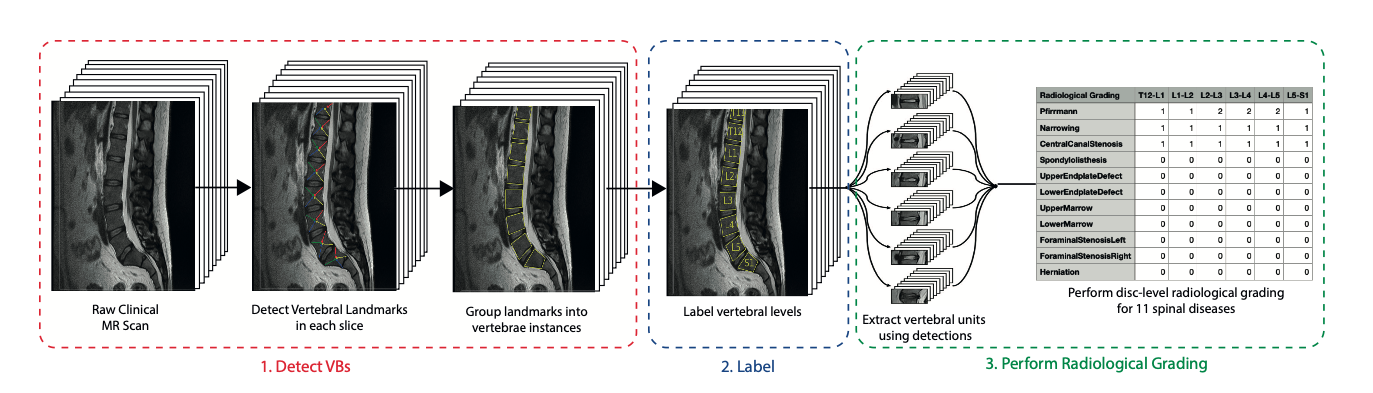
\includegraphics[width=\textwidth]{image/spinetv2_full_pipeline.png}
    \caption{Pipeline xử lý gốc của SpineNetV2~\cite{windsor2022spinenetv2}: phát hiện mốc đốt sống $\rightarrow$ gom thành đốt sống $\rightarrow$ gán mức $\rightarrow$ định vị khối liên đốt sống (IVV) $\rightarrow$ grading trên IVV.}
\end{figure}
\end{frame}

\begin{frame}
\frametitle{Phụ lục: phân bố nhãn trên SPIDER}
\begin{figure}
    \centering
    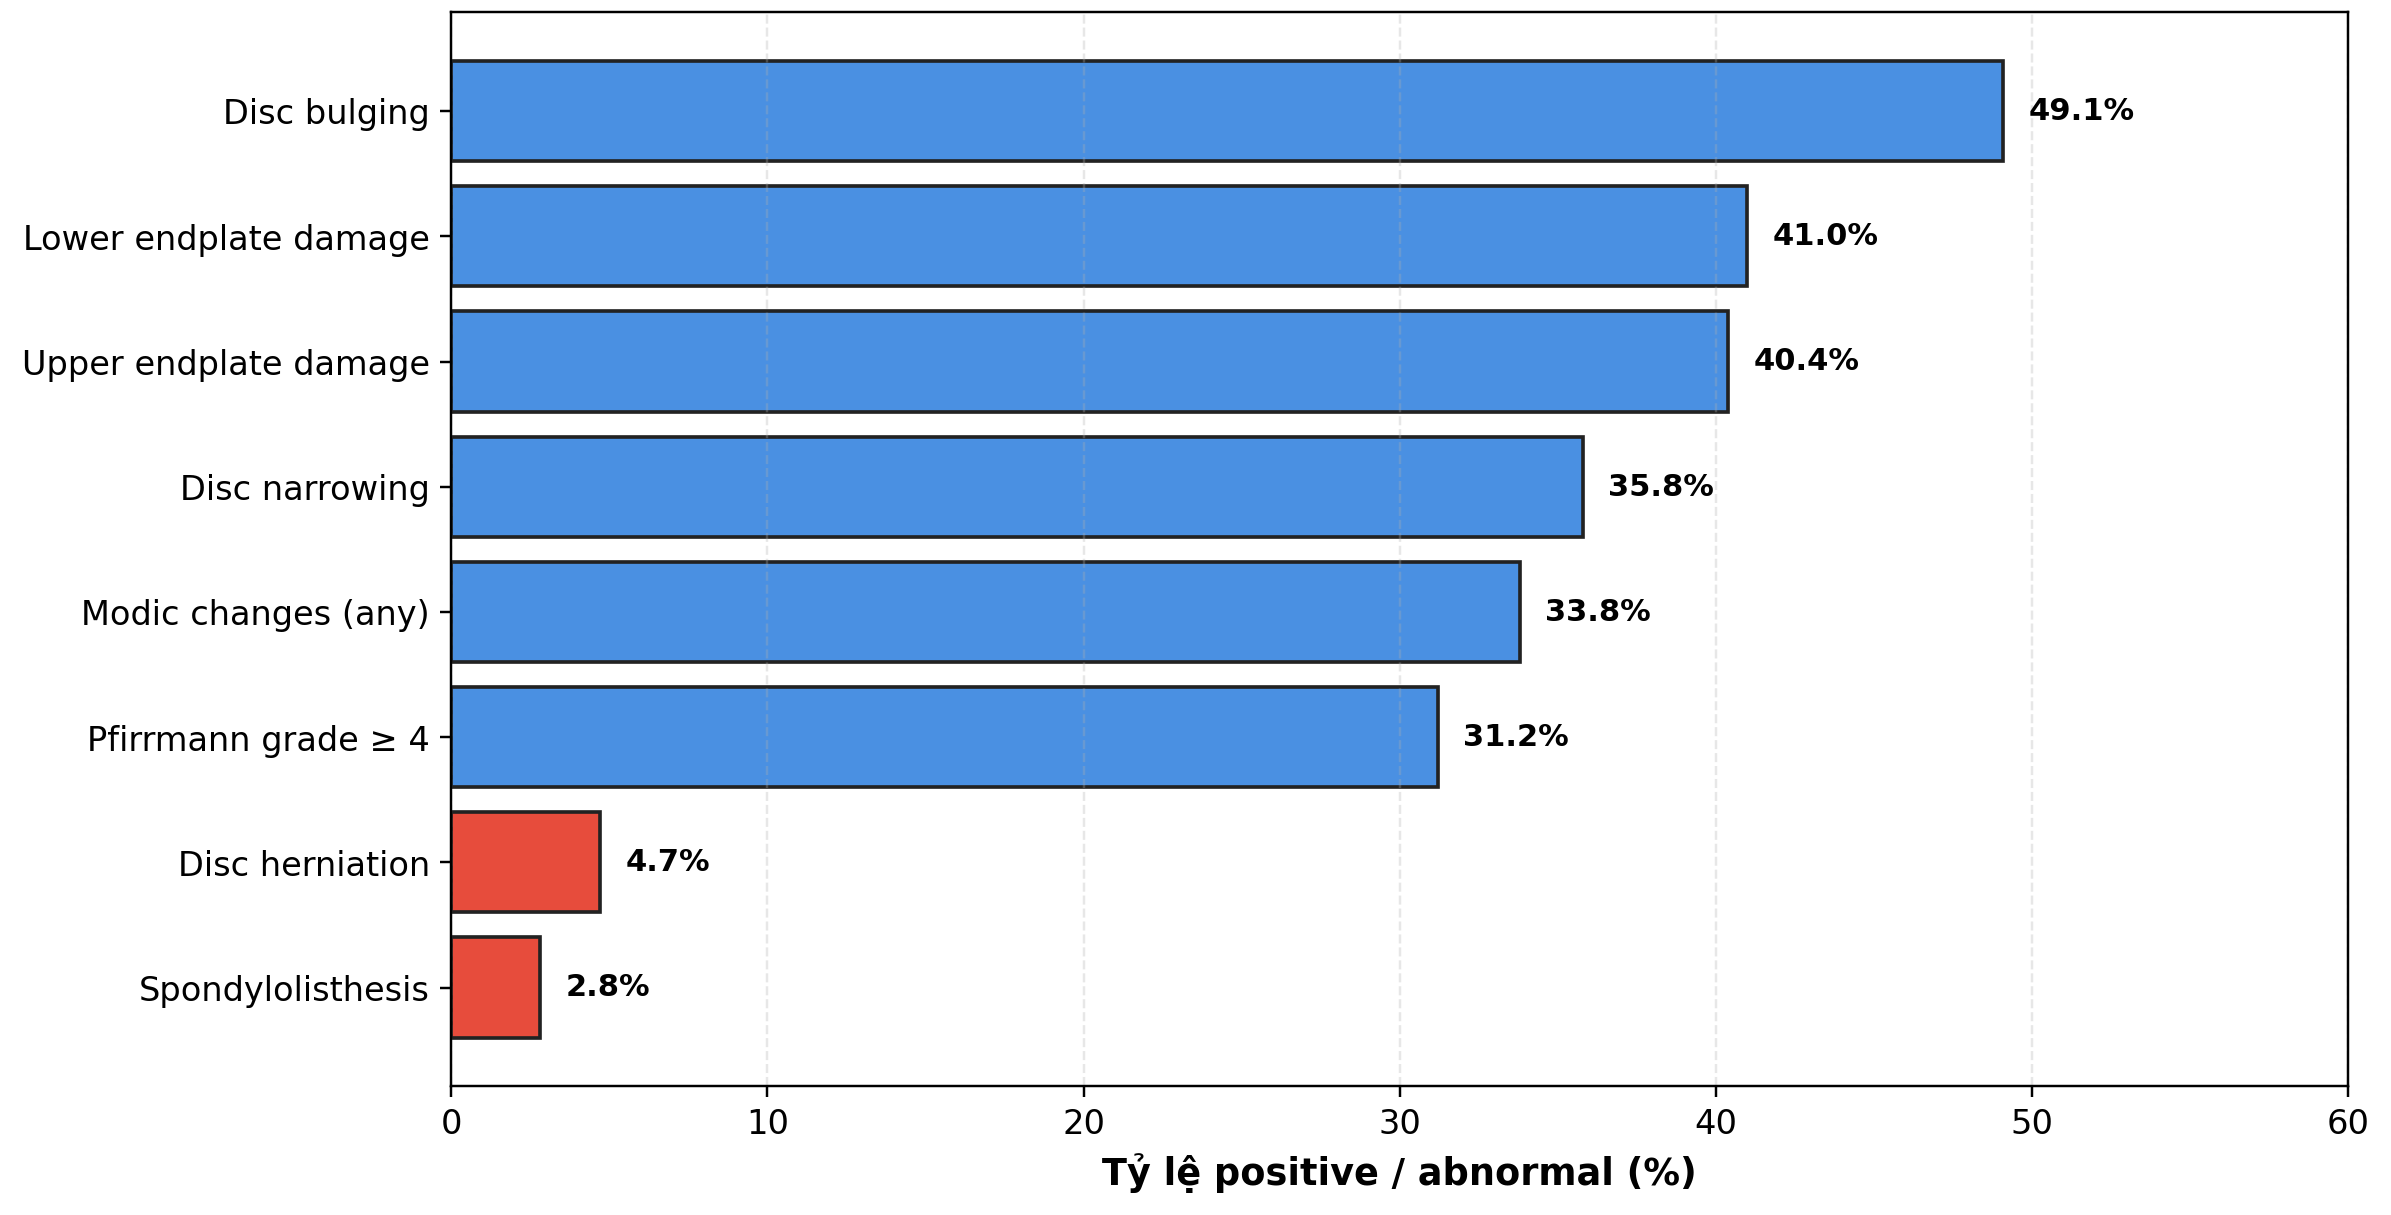
\includegraphics[width=0.82\textwidth]{image/spider_class_distribution.png}
    \caption{Phân bố nhãn trên SPIDER (8 nhóm bệnh) dùng để kiểm chứng tổng quát hóa.}
\end{figure}
\end{frame}

\end{document}
